\documentclass[tikz,border=4pt]{standalone}
\usepackage[T1]{fontenc}
\usepackage{lmodern}
\usepackage{amsmath}
\usetikzlibrary{arrows.meta,positioning,calc}

\definecolor{ink}{HTML}{334155}
\definecolor{learnededge}{HTML}{386C98}
\definecolor{learnedfill}{HTML}{EDF4FB}
\definecolor{fixededge}{HTML}{AD7B38}
\definecolor{fixedfill}{HTML}{FCF5E9}
\definecolor{outputedge}{HTML}{397866}
\definecolor{outputfill}{HTML}{EDF7F1}

\begin{document}
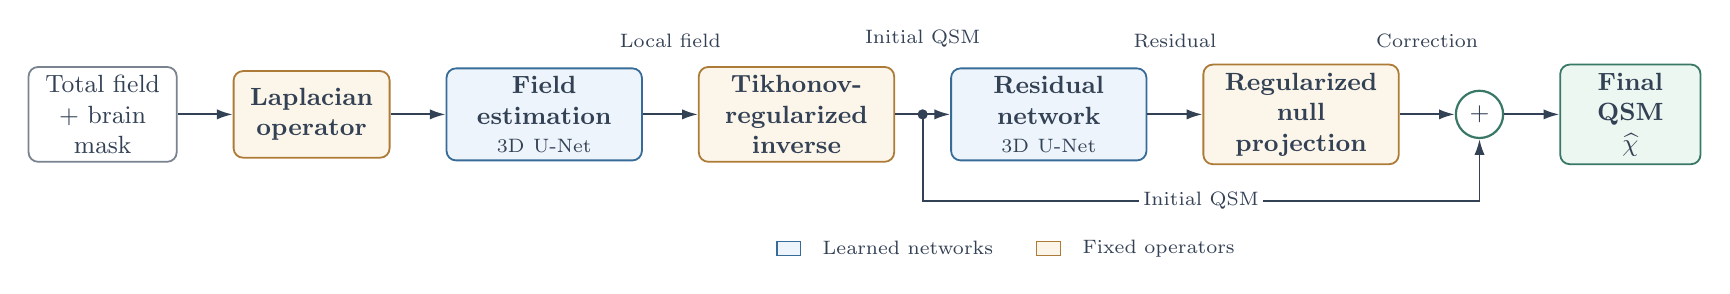
\begin{tikzpicture}[
    font=\small,
    text=ink,
    box/.style={
        draw=ink!65, line width=.65pt, rounded corners=1.2mm,
        minimum height=11mm, align=center, inner xsep=4pt, inner ysep=3pt
    },
    learned/.style={box,draw=learnededge,fill=learnedfill,text width=22mm},
    fixed/.style={box,draw=fixededge,fill=fixedfill,text width=17mm},
    flow/.style={-{Latex[length=2mm,width=1.3mm]},line width=.7pt,draw=ink},
    edge label/.style={font=\scriptsize,above=8mm,inner sep=1pt},
    legend text/.style={font=\scriptsize,anchor=west}
]
    \node[box,text width=16mm] (input) {Total field\\+ brain mask};
    \node[fixed,right=7mm of input] (laplacian)
        {\textbf{Laplacian}\\\textbf{operator}};
    \node[learned,right=7mm of laplacian] (field) {\textbf{Field}\\\textbf{estimation}\\[-1pt]{\scriptsize 3D U-Net}};
    \node[fixed,text width=22mm,right=7mm of field] (inverse)
        {\textbf{Tikhonov-}\\\textbf{regularized}\\\textbf{inverse}};
    \node[learned,right=7mm of inverse] (residual) {\textbf{Residual network}\\[-1pt]{\scriptsize 3D U-Net}};
    \node[fixed,text width=22mm,right=7mm of residual] (weight)
        {\textbf{Regularized}\\\textbf{null}\\\textbf{projection}};
    \node[circle,draw=outputedge,line width=.8pt,minimum size=6mm,
          inner sep=0pt,right=7mm of weight] (add) {$+$};
    \node[box,draw=outputedge,fill=outputfill,text width=15mm,
          right=7mm of add] (output) {\textbf{Final QSM}\\$\widehat\chi$};

    \draw[flow] (input) -- (laplacian);
    \draw[flow] (laplacian) -- (field);
    \draw[flow] (field) -- node[edge label] {Local field} (inverse);
    \draw[flow] (inverse) -- node[edge label] {Initial QSM}
        coordinate[midway] (initial) (residual);
    \draw[flow] (residual) -- node[edge label] {Residual} (weight);
    \draw[flow] (weight) -- node[edge label] {Correction} (add);
    \draw[flow] (add) -- (output);

    \fill[ink] (initial) circle (.65mm);
    \coordinate (skip) at ($(initial)+(0,-11mm)$);
    \draw[flow] (initial) -- (skip) -| (add.south);
    \node[font=\scriptsize,fill=white,inner sep=1.5pt]
        at ($(skip)!.5!(add |- skip)$) {Initial QSM};

    \coordinate (legend) at ($(field.center)!.5!(weight.center)+(0,-17mm)$);
    \node[draw=learnededge,fill=learnedfill,minimum width=3mm,
          minimum height=1.8mm,inner sep=0pt] (learnedkey)
        at ($(legend)+(-17mm,0)$) {};
    \node[legend text,right=1.5mm of learnedkey] {Learned networks};
    \node[draw=fixededge,fill=fixedfill,minimum width=3mm,
          minimum height=1.8mm,inner sep=0pt] (fixedkey)
        at ($(legend)+(16mm,0)$) {};
    \node[legend text,right=1.5mm of fixedkey] {Fixed operators};
\end{tikzpicture}
\end{document}
